\appendix

\begin{comment}
\chapter{Derivation of $A_v$}
\label{app:deriv_Av}

\chapter{OPAMP examples}
\label{app:opamp_examples}
\begin{minipage}{.4\textwidth}
	\centering
	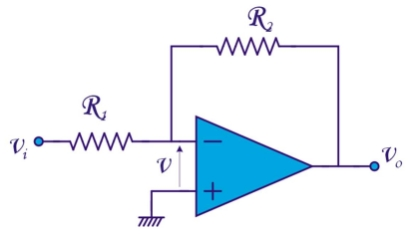
\includegraphics[width=6cm]{figures/ch02/opamp3.jpg}
\end{minipage}%
\begin{minipage}{.6\textwidth}
	\centering
	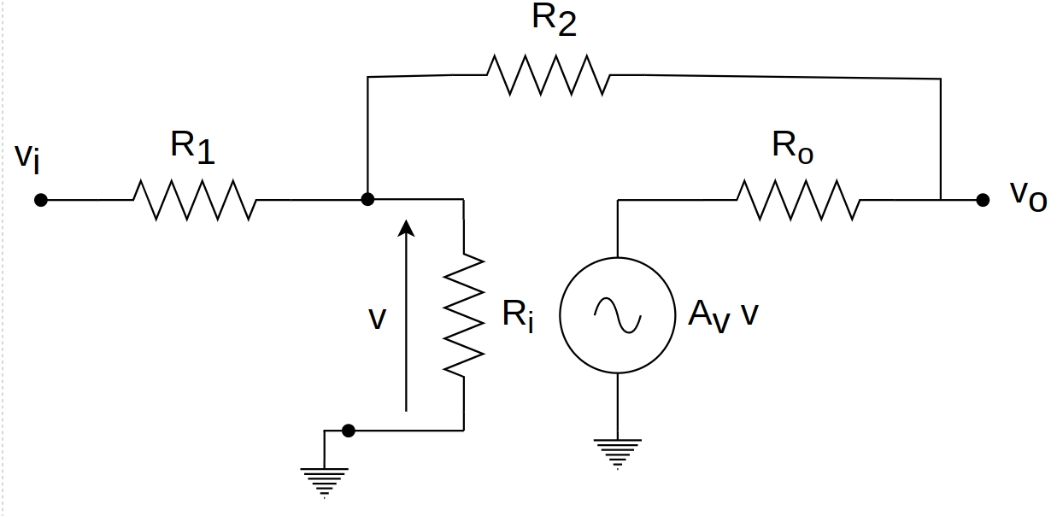
\includegraphics[width=8cm]{figures/app/opamp_inv.jpg}
\end{minipage}
\\
\begin{minipage}{.4\textwidth}
	\begin{itemize}
		\item $A_v$: $Z_i = \infty, R_o = 0$ 
		\begin{align*}
			v_o &= A_v v\\
			v   &= \frac{G_1 v_i + G_2 v_o}{G_1 + G_2} \\
			\Rightarrow v_o &= A_v \frac{G_1 v_i + G_2 v_o}{G_1 + G_2}  \\
			\Rightarrow v_o &= \frac{A_v G_1}{G_1 + G_2 - A_v G2} v_i \\
							&\approx -\frac{G_1}{G2} v_i =  -\frac{R_2}{R_1} v_i 
		\end{align*}
	\end{itemize}
\end{minipage}%
\begin{minipage}{.4\textwidth}
		\begin{itemize}
		\item $Z_{in}$: $A_v \rightarrow \infty \Rightarrow v = 0$
		\begin{align*}
			i_{in}  &= \frac{v_i - v}{R_1} \\
					&= \frac{v_i}{R_1}\\
			Z_{in} &= R_1
		\end{align*}
		\item $Z_{out}$: $R_i = \infty$\\
						 $ A_v \ne \infty, R_o \ne 0, v_i = 0$
		\begin{align*}
			v		 &= (R_1 || R_i) i_{out}  \approx R_1 i_{out} \\
			i_{out}  &= G_o (v_o - A_v v) + G_2 (v_o - v) \\
					 &= G_o (v_o - A_v R_1 i_{out}) + G_2 (v_o - R_1 i_{out})\\
					 &= \frac{G_o + G_2}{1 + A_v G_o R_1 + G_2 R_1} v_o\\
					 &= \frac{R_o + R_2}{R_o R_2 + A_v R_2 R_1 + R_o R_1} v_o\\
					 &\approx \frac{1}{A_v} \frac{R_o + R_2}{R_2 R_1} v_o\\
			\rightarrow Z_{out} &= A_v \frac{R_2 R_1}{R_o + R_2} \approx A_v R_1 \\
		\end{align*}
	\end{itemize}
\end{minipage}
\\ TODO: check this

\begin{minipage}{.4\textwidth}
	\centering
	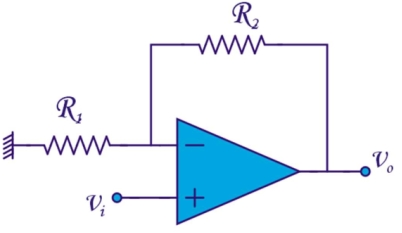
\includegraphics[width=6cm]{figures/ch02/opamp4.jpg}
\end{minipage}%
\begin{minipage}{.6\textwidth}
	\centering
	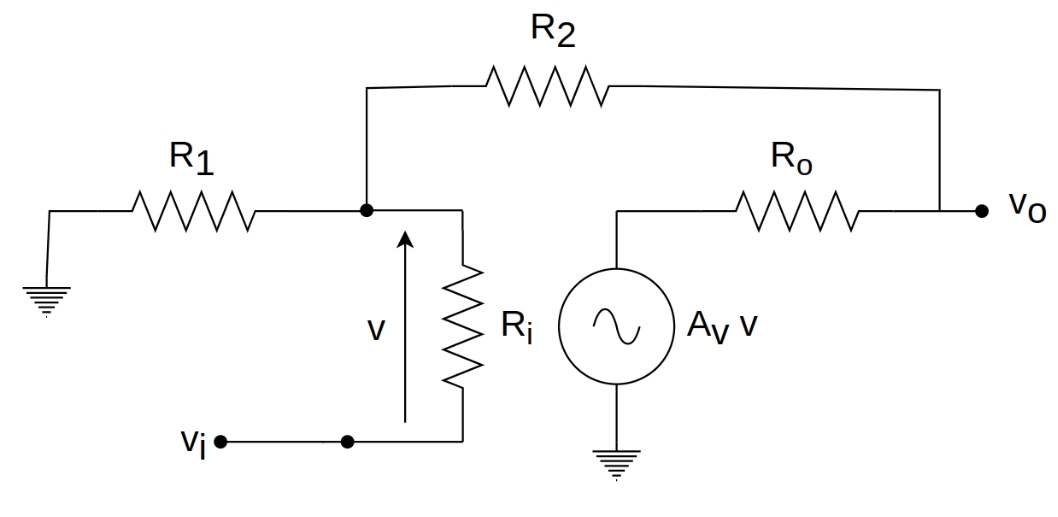
\includegraphics[width=8cm]{figures/app/opamp_noninv.jpg}
\end{minipage}

\begin{minipage}{.4\textwidth}
	\centering
	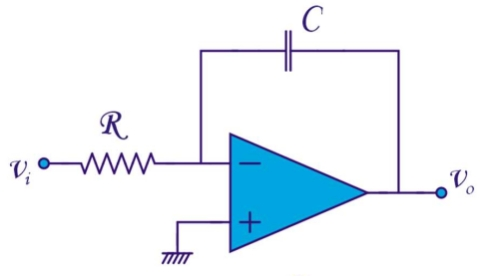
\includegraphics[width=6cm]{figures/app/opamp_ex1.jpg}
\end{minipage}%
\begin{minipage}{.6\textwidth}
	\centering
	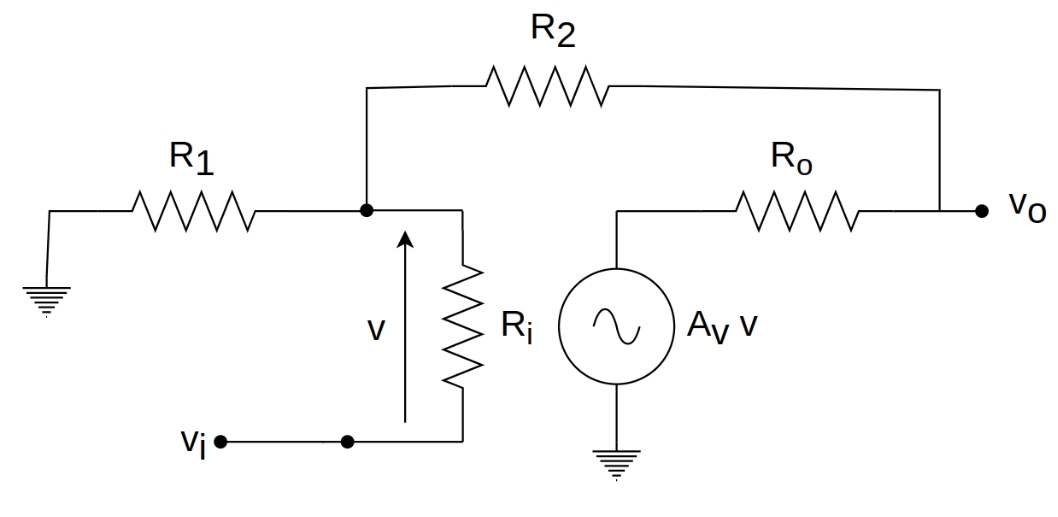
\includegraphics[width=8cm]{figures/app/opamp_noninv.jpg}
\end{minipage}

\begin{minipage}{.4\textwidth}
	\centering
	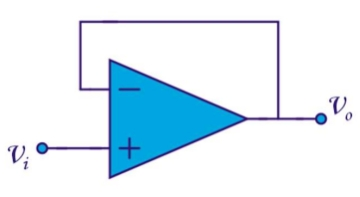
\includegraphics[width=6cm]{figures/app/opamp_ex2.jpg}
\end{minipage}%
\begin{minipage}{.6\textwidth}
	\centering
	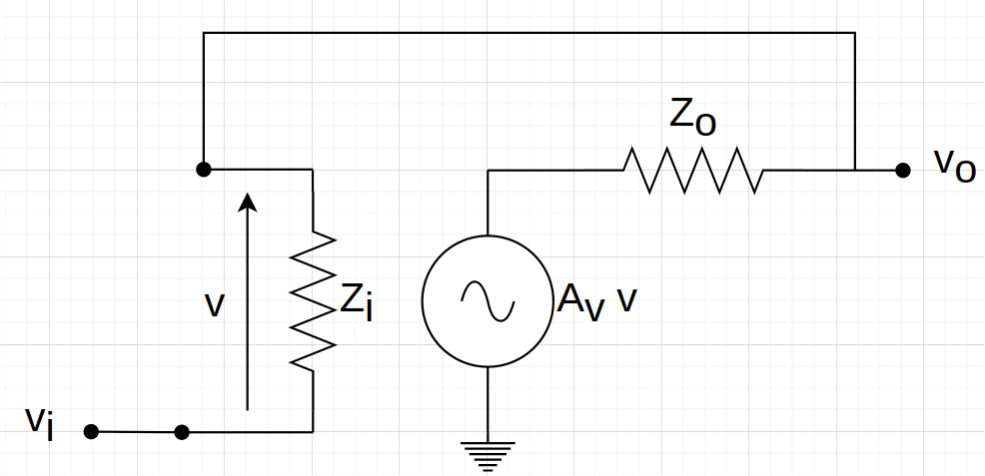
\includegraphics[width=8cm]{figures/app/opamp_ex3b.jpg}
\end{minipage}

\begin{minipage}{.4\textwidth}
	\centering
	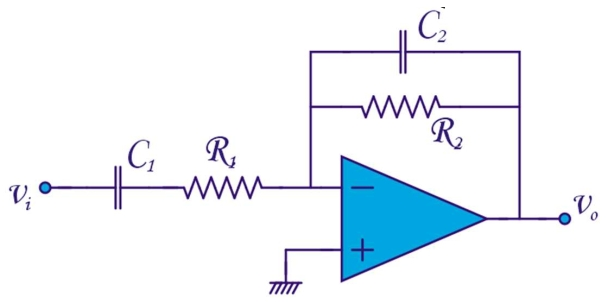
\includegraphics[width=6cm]{figures/app/opamp_ex3.jpg}
\end{minipage}%
\begin{minipage}{.6\textwidth}
	\centering
	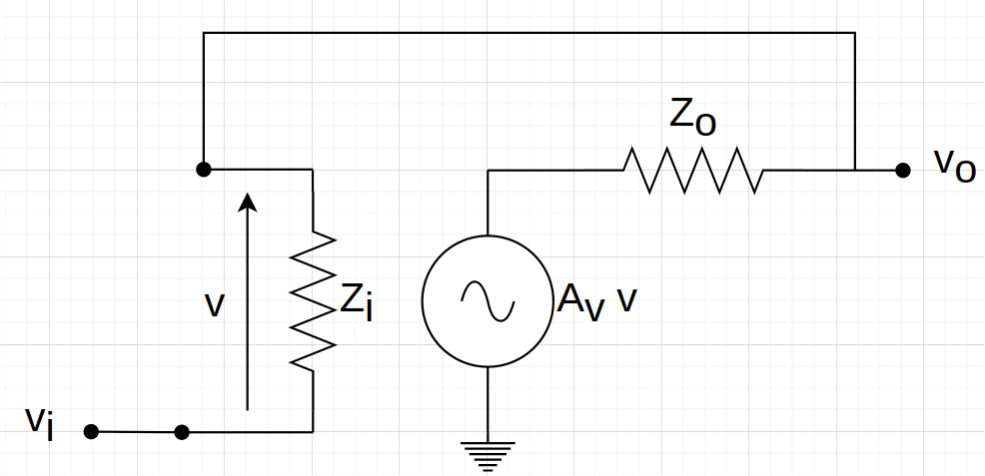
\includegraphics[width=8cm]{figures/app/opamp_ex3b.jpg}
\end{minipage}


\chapter{Sequential Design Examples}
\label{app:design_examples}
\end{comment}

\chapter{Exam Questions}
\label{app:exam_questions}
	\begin{enumerate}
	\item Discuss the PN-junction, including the small-signal model (\ref{ch:pnjunction} and \ref{sec:small_signal_response})
	\item Discuss the BJT, including the small-signal model (\ref{sec:bipolar_junction} and \ref{sec:bjt_small_signal})
	\item Discuss the MOSFET,  including the small-signal model (\ref{sec:mosfet} and \ref{sec:mosfet_small_signal})
	\item Discuss the biasing of the BJT (\ref{sec:bjt_biasing})
	\item Discuss the biasing of the MOSFET (\ref{sec:mosfet_biasing})
	\item Discuss the four-resistor amplifier (\ref{sec:four_resistor})
	\item Discuss the common emitter/source amplifier (\ref{sec:cea})
	\item Discuss the common basis/gate amplifier (\ref{sec:cba})
	\item Discuss the common collector/drain amplifier (\ref{sec:cca})
	\item Discuss the differential amplifier (\ref{sec:diff_amplifier})
	\item Discuss the operational amplifier, including sources of error (\ref{sec:opamp})
	\item What is the Miller capacitor? (\ref{sec:miller_cap})
	\item Discuss the class A amplifier (\ref{sec:classA})
	\item Discuss the class B amplifier (\ref{sec:classB})
	\item Discuss the Push-Pull amplifier (\ref{sec:push_pull})
	\item Discuss the class C amplifier (\ref{sec:classC})
	\item Discuss the class S amplifier (\ref{sec:classS})
	\item Discuss the selective amplifier (\ref{sec:selective_amp})
	\item Discuss the impact of feedback (\ref{ch:feedback})
	\item Discuss the Wien Bridge oscillator (\ref{sec:wien_bridge})
	\item Discuss the Colpitts oscillator (\ref{sec:colpitts})
	\item Discuss the relaxation oscillator (\ref{sec:relaxation})
	\item Discuss the Fantastron (\ref{ch:fantastron})
	\item Discuss the diode rectifier (\ref{sec:diode_rectifier})
	\item Discuss the single  voltage stabilizer (\ref{sec:voltage_stabilizer})
	\item Discuss the voltage stabilizer with transistor (\ref{sec:transistor_stabilizer})
	\item Discuss transistor-transistor logic (\ref{sec:ttl})
	\item Discuss emitter-coupled logic (\ref{sec:ecl})
	\item Discuss the Schmidt trigger (\ref{sec:schmidt})
	\item Discuss the edge-triggered D-latch (\ref{sec:dlatch})
	\item Discuss the sequential design procedure (\ref{sec:seq_design})
	\item Discuss the R-2R DAC (\ref{sec:dac_voltage_distribution})
	\item Discuss the DAC with charge distribution (\ref{sec:charge_distribution})
	\item Discuss the serial ADC with single and double integration (\ref{sec:serial_adc})
	\item Discuss the SAR and Flash converter (\ref{sec:sar} and \ref{sec:flash})
\end{enumerate}